\section{Implementation}
Matadorspillet er udelukkende skrevet i Java og vi har benyttet os af Intellij som IDE. Matadorspillet er opbygget af klasser, som vi har benyttet Java til at lave. \\
Der er tager brug af biblioteket Diplomitdtu:matadorgui version 3.1.7, hvilket GUIen er oprettet og bliver vist igennem. Da GUIen bliver fremvist ved hjælp af biblioteket, har vi, som programmører primært, skulle skrive logikken til spillet uden at fokusere på, hvordan det bliver vist for brugeren. Dette har vi gjort igennem 8 forskellige klasser, som sammen kommunikerer med biblioteket for at vi Matadorspillet til at fungere.
De forskellige klasser er forklaret nedenfor.\\
Et Javadoc til biblioteket kan findes i reference \cite{javadoc}. 
\\

\subsection{Spillets klasser}

\subsubsection{Main}
Main er en helt central klasse i programmet. Det er primært denne klasse som kommunikerer med GUIen. Derudover tager den brug af de fleste metoder fra de andre klasser. Da Main er så central i vores program, har vi valgt at oprette de fleste elementer, derunder variabler, arrays og objekter som public, så de kan tilgås fra de tilhørende klasser. Igennem kommunikation med biblioteket, bliver spillerne, spillepladen og felterne oprettet i Main.\\
I denne klasse bliver spillets primære loop også kørt. Loopet skifter mellem de forskellige spillere, og styrer bland andet hvornår en spiller skal kaste en terning, rykke og evt. betale eller medtage penge. Når dette loop bliver brudt, er spillet slut og en taber og evt. vinder vil findes.

\subsubsection{FeltLogik}
Feltlogik klassen er en public klasse, som extender mMin, for at kunne tilgå visse objekter oprettet i Main klassen. FeltLogik klassen bruges i sammenhæng med Main klassen til, at finde ud af, hvilket felt den enkelte spiller befinder sig på, tjekke hvorvidt feltet er ejet af en anden spiller, hvem der ejer det enkelte fag samt at rykke spilleren rundt på de forskellige felter. Derudover hjælper klassen også med, at rykke spilleren i fængsel, hvis spilleren har ramt feltet "Gå i fængsel". I klassen er der ingen variable som er oprettet til brug af hele klassen, men i stedet kun for de enkelte metoder. Variablerne er altså oprettet lokalt i de metoder som benytter dem.

\subsubsection{Spiller}
Spiller klassen har udelukkende forbindelse til Main klassen. Klassen holder styr på spillernes navne, antallet af spillere samt spillernes indledende balance. Klassen har 2 public variabler af hhv. et String array til spillernes navne, og en enkelt int til antallet af spillere. Disse to variabler er gjort public, da de begge bliver brugt inde i Main. Spiller klassen tager brug af bibliotekets GUI del, da der her bliver fremvist tekst-input felter til spillernes navne.

\subsubsection{Logik}
Logik klassen er en public klasse, som extender Main. Klassen extender Main, da klassen ikke ville kunne bruges eller fungere uden visse oprettede elementer i main, og det er derfor nødvendigt for Logik at Main findes. Denne klasse er blevet oprettet for, at fordele de mange metoder vores program tager brug af, ud i flere kategorier. Logik er altså klassen hvor de variabler som ikke gav mening af oprette inde i enten FeltLogik eller Spiller. Med Logik klassen er det muligt, at finde både vinder og taber samt køb af felt og betaling mellem to spillere.

\subsubsection{ChanceKort}
ChanceKort klassen er en meget simpel klasse, som bruges til at henvise videre til metoderne i RunChanceKort. Klassen er en public class hvis formål er, at finde et tilfældigt chancekort og initialisere metoden inde i RunChanceKort ved hjælp af en simpel switch.

\subsubsection{RunChanceKort}
RunChanceKort indeholder alle spillets chancekort, deres tekst og deres logik, og har mulighed for at fremvise chancekortne i GUIen når nødvendigt. Hvert chancekort er altså i stand til, at både rykke spillerne rundt på pladen, få spillere ud af fængslet samt give og trække penge på de respektive konti.

\subsubsection{Felter}
Felter klassen består udelukkende af et array af felterne på spillerpladen. Ved hjælp af det importerede matador bibliotek, bliver hvert felt oprettet som et objekt med en række variabler der kan angives ved start. Da denne klasse ikke på noget tidspunkt ændrer sig, er klassen oprettet som public final og dets variabler er oprettet som private final. Alle variabler i denne klasse er udelukkende brugt i klassen selv.

\subsubsection{Dice}
Dice klassen er en public klasse hvis formål er at kaste terningen og derved finde et random tal mellem 1 og 6. Hvis man ønsker at ændre terningen til en større type terning, kan dette nemt ændres ved at ændre klassens MAX værdi. Terningen bliver udelukkende brugt til, at angive hvor mange felter spilleren skal rykke på brættet.

 

\subsection{Versionsstyring}
Versionsstyring foregår igennem GIT ved brug af Github som fjern repository. Ved udvikling af dette projekt har vi benyttet os af flere branches til forskellige dele af projektet. Der er bl.a. blevet oprettet en \emph{udviklings branch}, som vi har benyttet til at skrive koden i. Når et stykke kode er skrevet i udviklings-branchen, har vi herefter oprettet \emph{Release branch}, hvor de forskellige dele af programmet samles sammen. Her testes der om programmet nu virker samlet og er dette tilfældet, bliver hele programmet merget ind \emph{master branch}, som nu danner baggrund for det færdig udviklet program.
\\Derudover er der også oprettet en \emph{feature branch}, som kan benyttes til at skrive ny kode og teste forskellige scenarier, som går ud over projektbeskrivelsen, uden at det har indflydelse på det færdig skrevet kode.

\begin{figure}[H]
        \centering
        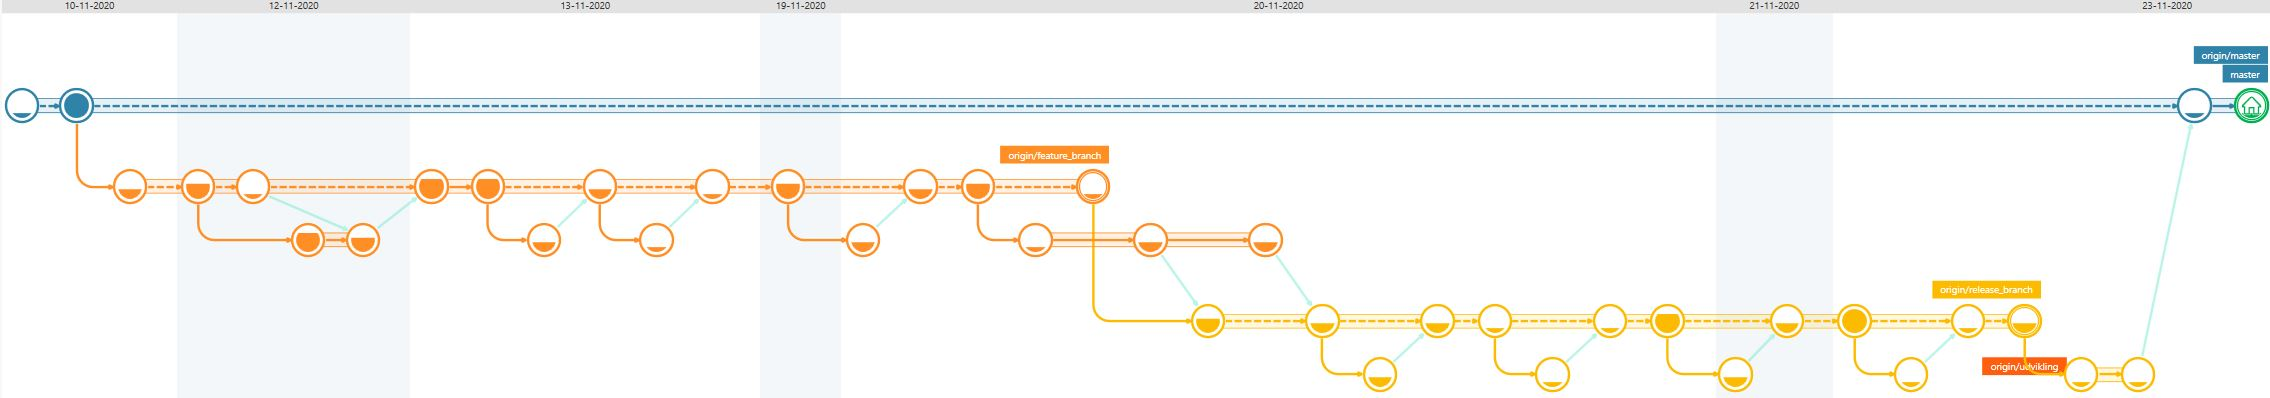
\includegraphics[width=17cm]{figures/gitVisualize.JPG}
        \caption{Git Visualization with GMaster}
    \end{figure}
    